\chapter{Introduction to mobile robotics}
\label{chap:robotics}
  Human beings always created tools to make its job easier. 
  Even the word "robot", first used by Karel �apek in a novel RUR published in 1920, came from world "robota", 
  which in Czech means labour.

  \begin{figure}[!hbp]
  \centering
  \ifpdf
    \setlength{\unitlength}{1bp}%
    \begin{picture}(188.50, 153.07)(0,0)
    \put(0,0){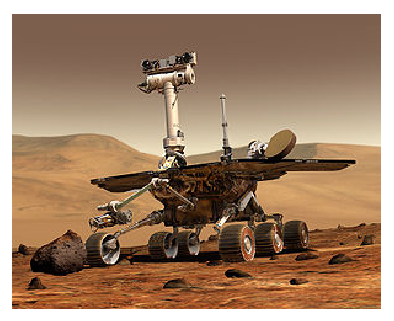
\includegraphics{spirit_rover.pdf}}
    \end{picture}%
  \else
    \setlength{\unitlength}{1bp}%
    \begin{picture}(188.50, 153.07)(0,0)
    \put(0,0){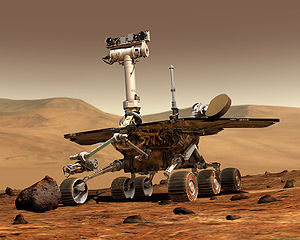
\includegraphics{spirit_rover}}
    \end{picture}%
  \fi
  \caption{\label{pic:spirit_rover}%
   Rover Spirit on Mars}
  \end{figure}
  %\input{spirit_rover.TpX}%Rover Spirit on Mars

  Nowadays mobile robots are useful in many areas. Robots excel in exploration of danger places. 
  For example rover Spirit and Delta II flew to Mars. Spirit is a robot of our imagination. It is a six wheel robot
  which is similar to police robots for a bomb manipulation.
  On the other hand, Delta II is a space rocket. 
  Robots like Delta II and Spirit allow humankind to explore so distant places, which are too far for a man to travel there.
  
  However, mobile robots are not narrow specialised in adventurous actions and missions impossible for humans. 
  Their main contribution is in daily life.
  In many cities of the world the robots are used in public transport. They drive the trains in metro,
  help pilots to take off or land planes. They are used to park cars or they control cruise controls.
  Solutions which were studied in mobile robotics are usually incorporated in daily life use. 
  One time a car computer helps to park a car,
  another time a vacuum cleaner tidies up a room.
  Robots are useful not only as independent machines. Most of the robots help people with difficult tasks, 
  but people control their actions directly.
  Nice example is a parking robot present in many contemporary cars.
  
  On the other hand, the research in mobile robotics tries to produce robots which are autonomous as much as possible.
  The developers transfer all control to a robot, which is particularly demanding if the robot interacts with people. 
  There are areas where the research and industry already succeed.
  
  %\input{aibo.TpX}
  \begin{figure}[!hbp]
  \centering
  \ifpdf
    \setlength{\unitlength}{1bp}%
    \begin{picture}(241.89, 184.25)(0,0)
    \put(0,0){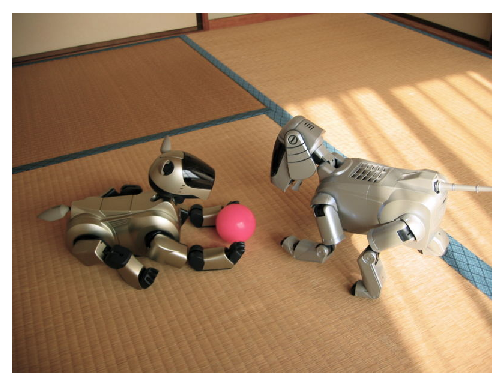
\includegraphics{aibo.pdf}}
    \end{picture}%
  \else
    \setlength{\unitlength}{1bp}%
    \begin{picture}(241.89, 184.25)(0,0)
    \put(0,0){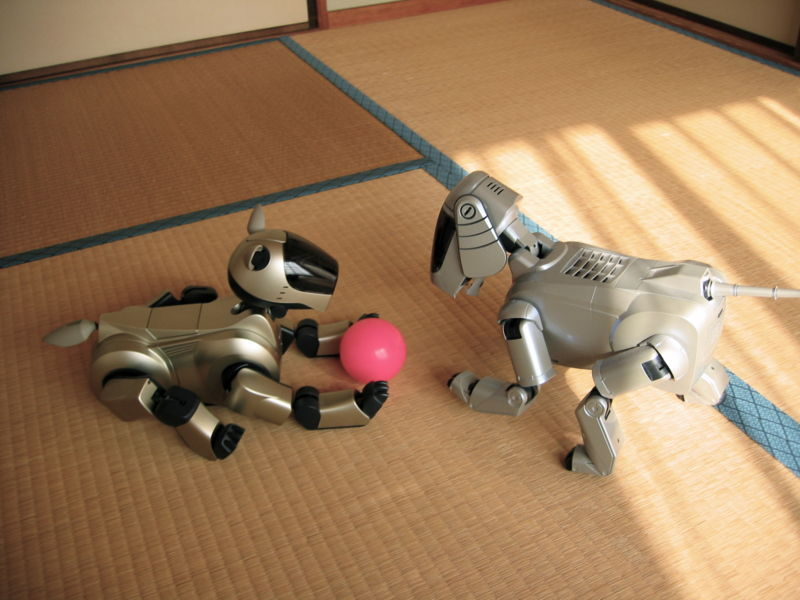
\includegraphics{aibo}}
    \end{picture}%
  \fi
  \caption{\label{pic:aibo}%
   Two versions of an Aibo robot}
  \begin{quote}
  "About 4.4 million units for domestic use and about 2.8 million units for entertainment and leisure sold up to end 2009."
  \cite{worldrob}
  \end{quote}
  \end{figure}
  Autonomous vacuum cleaners and lawnmowers are broadly used in households and in gardens
  and no one has fear from them.
  A number of robotic toys have been already sold.
  A robotic dog Aibo introduced in 1999 is a nice example of a toy robot.
  
  Not only entertainment robots are designed for human-robot interaction. In Japan there is a big stress 
  on creating	robots for health care, which will compensate lack of medical personnel. 
  A robot has to be a humanoid, because especially children and older people are used to 
  communicate with other people and not with machines.
  
  Professor Hiroshi Ishiguro from Japan reached a great success in field of humanoid robots. 
  His goal is to build robot, which would be a good companion for a human. 
  Among other humanoids he has successfully constructed a copy of himself.
%  Hiroshi Ishiguro is concentrating on simulating human behaviour, speech and motion, 
%  but he also invented a touch sensor, which substitutes human skin on his robots.
  %\input{ishiguro_clone.TpX}%Ishiguro with his humanoid
  \begin{figure}[!hbp]
  \centering
  \ifpdf
    \setlength{\unitlength}{1bp}%
    \begin{picture}(148.82, 213.43)(0,0)
    \put(0,0){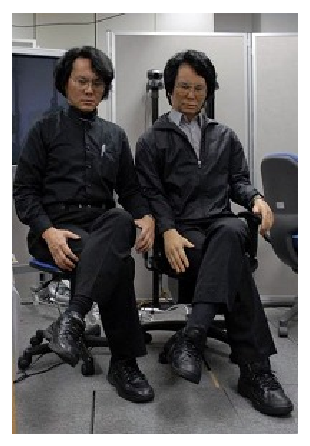
\includegraphics{ishiguro_clone.pdf}}
    \end{picture}%
  \else
    \setlength{\unitlength}{1bp}%
    \begin{picture}(148.82, 213.43)(0,0)
    \put(0,0){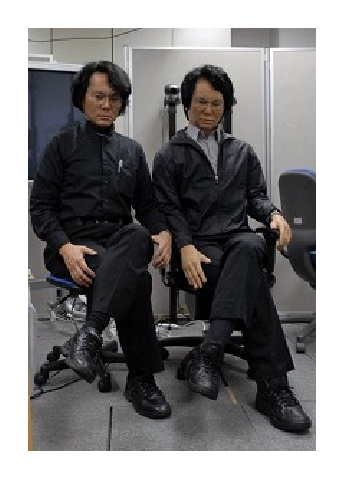
\includegraphics{ishiguro_clone}}
    \end{picture}%
  \fi
  \caption{\label{pic:ishigure_clone}%
   Ishiguro and his humanoid}
  \end{figure}
	
  The humanoid robots and also the Aibo robot are not  wheeled robots, although the wheeled 
  robotic systems are still dominating. The reason is in the field of the activity of the robots. 
  The entertainment and the health care robots are in the human environment. 
  Robots avoid a lot of different obstacles and they have to use stairs.
  The industrial robots are usually indoors, where the terrain is adapted to machines movement. 
  Also the agricultural robots have convenient conditions for wheel movement.
  
  Not only the design of robots, but also the control of robots differs and evolves.
  In the eighties the sense-plan-act model was current.
  Later in the nighties the behaviour model was introduced by Brooks,
  which was a very modern and sometimes strictly implemented.	
  After a decade a compromise between the behaviour based robotics and the simple planning was popular.
  In the nighties neural networks and other modern, biologically motivated attitudes were first introduced.
  Genetic algorithms and neural networks have enormous success in solving complicated control problems like motion of
  robot with a number of legs, implementing very sophisticated behaviour and so on.
  
  To conclude, mobile robotics is a dynamically evolving science,
  which has all preconditions to be one of the leading research areas in the twenty first century.
  The value of the market increased to 6.2 billion dollars in 2009 according to the International Federation of Robotics.
  \cite{worldrob}
  \begin{quote}	 	
  "I can envision a future in which robotic devices will become a nearly ubiquitous part of our day-to-day lives," 
  \end{quote}
  says Bill Gates, who was at the beginning of the computer revolution. %todo citation?
  



